\documentclass[tikz]{standalone}

\usepackage{tikz}
\usetikzlibrary{trees}
\usetikzlibrary{shapes}
\usetikzlibrary{positioning}
\usetikzlibrary{arrows.meta}

\tikzset{
    pointer/.style = {thick,draw=black,triangle 45-*,shorten >=-3pt},
    cell/.style = {rectangle, thick, draw=black,minimum width = 1cm, minimum height =1.0cm,fill=yellow!20},
    mynode/.style = {circle, thick, draw=black, align=center,fill=yellow!40,font=\ttfamily\bfseries\Large},
    mynoder/.style = {circle, thick, draw=black, align=center,fill=red!30,font=\ttfamily\bfseries\Large},
    mynodeb/.style = {circle, thick, draw=black, align=center,fill=blue!30,font=\ttfamily\bfseries\Large},
    edgen/.style = {-latex,ultra thick},
    edger/.style = {-latex,ultra thick,red},
    edgeb/.style = {-latex,ultra thick,blue},
    edgeg/.style = {-latex,ultra thick,gray},
    edgegd/.style = {-latex,ultra thick,brown,dashed}, % back
    edgevd/.style = {-latex,ultra thick,violet,dotted}, % forward
    edgexd/.style = {-latex,ultra thick,blue,densely dotted}, % traversal
    every picture/.style={/utils/exec={\ttfamily\bfseries}},
    every picture/.style={font issue=\ttfamily\bfseries},
    font issue/.style={execute at begin picture={#1\selectfont}
  }
}

\begin{document}



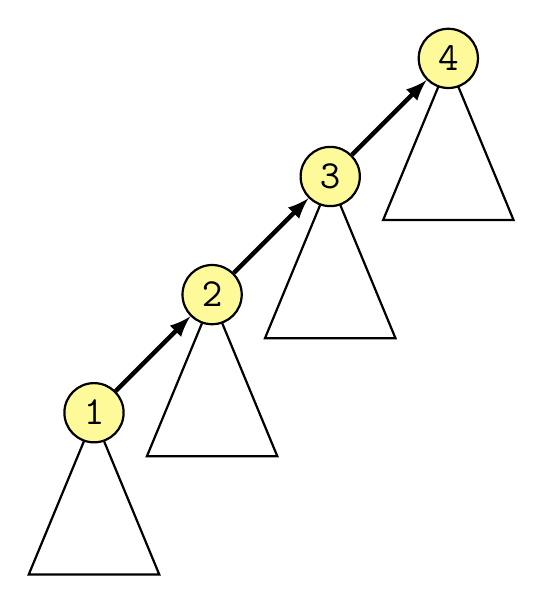
\begin{tikzpicture}[thick,font=\ttfamily\bfseries,
    triangle/.style={isosceles triangle,draw,shape border rotate=90, minimum height=20mm, minimum width=10mm, inner sep=0,fill=white},
]
\node[triangle] at (0.0, -1.5) {};
\node[triangle] at (1.5, 0.0) {};
\node[triangle] at (3.0, 1.5) {};
\node[triangle] at (4.5, 3.0) {};
\node[mynode] at (0.0, 0.0) (a) {1};
\node[mynode] at (1.5, 1.5) (b) {2};
\node[mynode] at (3.0, 3.0) (c) {3};
\node[mynode] at (4.5, 4.5) (d) {4};
%
\draw[edgen] (a) edge node {} (b);
\draw[edgen] (b) edge node {} (c);
\draw[edgen] (c) edge node {} (d);

\end{tikzpicture}


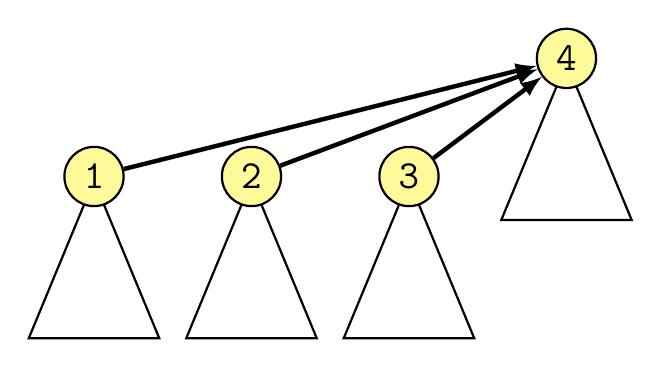
\begin{tikzpicture}[thick,font=\ttfamily\bfseries,
    triangle/.style={isosceles triangle,draw,shape border rotate=90, minimum height=20mm, minimum width=10mm, inner sep=0,fill=white},
]

\node[triangle] at (8.0, 1.5) {};
\node[triangle] at (10.0, 1.5) {};
\node[triangle] at (12.0, 1.5) {};
\node[triangle] at (14.0, 3.0) {};
\node[mynode] at (8.0, 3.0) (a) {1};
\node[mynode] at (10.0, 3.0) (b) {2};
\node[mynode] at (12.0, 3.0) (c) {3};
\node[mynode] at (14.0, 4.5) (d) {4};
%
\draw[edgen] (a) edge node {} (d);
\draw[edgen] (b) edge node {} (d);
\draw[edgen] (c) edge node {} (d);

\end{tikzpicture}

\end{document}
